% Chapter 1

\chapter{Background and related work to the M/EEG inverse problem} % Main chapter title
\label{chapter:background} % For referencing the chapter elsewhere, use \ref{Chapter1} 
\noindent\makebox[\linewidth]{\rule{0.75\paperwidth}{0.4pt}}
\noindent\makebox[\linewidth]{\rule{0.75\paperwidth}{0.4pt}}

\localtableofcontents % local toc

\noindent\makebox[\linewidth]{\rule{0.75\paperwidth}{0.4pt}}
\noindent\makebox[\linewidth]{\rule{0.75\paperwidth}{0.4pt}}

\newpage
%----------------------------------------------------------------------------------------

% Define some commands to keep the formatting separated from the content 
\newcommand{\keyword}[1]{\textbf{#1}}
\newcommand{\tabhead}[1]{\textbf{#1}}
\newcommand{\code}[1]{\texttt{#1}}
\newcommand{\file}[1]{\texttt{\bfseries#1}}
\newcommand{\option}[1]{\texttt{\itshape#1}}


%--------- Signal sources of MEEG recording-----------------------------------------------
\section{Signal sources of MEG and EEG recordings}
%Measuring weak MEG/EEG signals in the background of strong environmental noise, having a noise level of several orders of magnitude larger than the MEG/EEG signals, is a challenging task. 
At the cellular level of the brain, its nervous system is defined by the presence of special type of neural cells. Despite the apparent simplicity in the structure of the neural cell, the biophysics of neural current flow relies on a complex network of billions of cells, neurons and glial cells~\cite{baillet2001electromagnetic, hodgkin1964conduction}. Neurons are nerve cells that transmit nerve signals to and from the brain, they are about 100 billions neurons. The neuron consists of a cell body (or soma) with branching dentrites (signal receivers). They send these signals in the form of electrochemical waves traveling along thin fibers called axons, which cause chemicals called neurotransmitters to be released at junctions called synapses. A cell that receives a synaptic signal from a neuron may be excited, inhibited, or otherwise modulated. At a synapse, the cell that sends signals is called presynaptic, and the cell that receives signals is called postsynaptic.\\

Every neuron maintains a voltage gradient across its membrane, due to metabolically-driven differences in ions of sodium, potassium, chloride and calcium within the cell, each of which has a different charge. If the voltage changes significantly, an electro-chemical pulse called an action potential (or nerve impulse) is generated. This electrical activity can be measured and displayed as a wave form called brain wave or brain rhythm. This pulse travels rapidly along the cell's axon, and is transferred across a synapse to a neighbouring neuron, which receives it through its feathery dendrites. Each individual neuron can form thousands of links with other neurons in this way, giving a typical brain well over 100 trillion synapses (up to 1,000 trillion, by some estimates).\\

Roughly, when a neuron is excited by other—and possibly remotely located—neurons via an afferent volley of action potentials, excitatory postsynaptic potentials (EPSPs) are generated at its apical dendritic tree. The apical dendritic membrane becomes transiently depolarized and consequently extracellularly electronegative with respect to the cell soma and the basal dendrites. This potential difference causes a current to flow through the volume conductor from the nonexcited membrane of the soma and basal dendrites to the apical dendritic tree sustaining the EPSPs~\cite{gloor1985neuronal}.
Some of the current takes the shortest route between the source and the sink by traveling within the dendritic trunk. Conservation of electric charges imposes that the current loop be closed with extracellular currents flowing even through the most distant part of the volume conductor. Intracellular currents are commonly called primary currents, while extracellular currents are known as secondary, return, or volume currents.\\

Both primary and secondary currents contribute to magnetic fields outside the head and to electric scalp potentials, but spatially structured arrangements of cells are of crucial importance to the superposition of neural currents such that they produce measurable fields. Tens of thousands of synchronously activated large pyramidal cortical neurons are thus believed to be the main MEG and EEG generators because of the coherent distribution of their large dendritic trunks locally oriented in parallel, and pointing perpendicularly to the cortical surface~\cite{nunez2000relationship}. The currents associated with the EPSPs generated among their dendrites are believed to be at the source of most of the signals detected in MEG and EEG because they typically last longer than the rapidly firing action potentials traveling along the axons of excited neurons~\cite{nunez2006electric}. %Indeed, calculations such as those shown in~\cite{hamalainen1993magnetoencephalography} suggest each synapse along a dendrite may contribute as little as a 20 fA-m current source, probably too small to measure in MEG/EEG. Empirical observations instead suggest we are seeing sources on the order of 10 nA-m, and hence the cumulative summation of millions of synaptic junctions in a relatively small region. Nominal calculations of neuronal density and cortical thickness suggest that the cortex has a macro-cellular current density on the order of 100 nA/mm2.\\

\begin{figure}
	\centering
	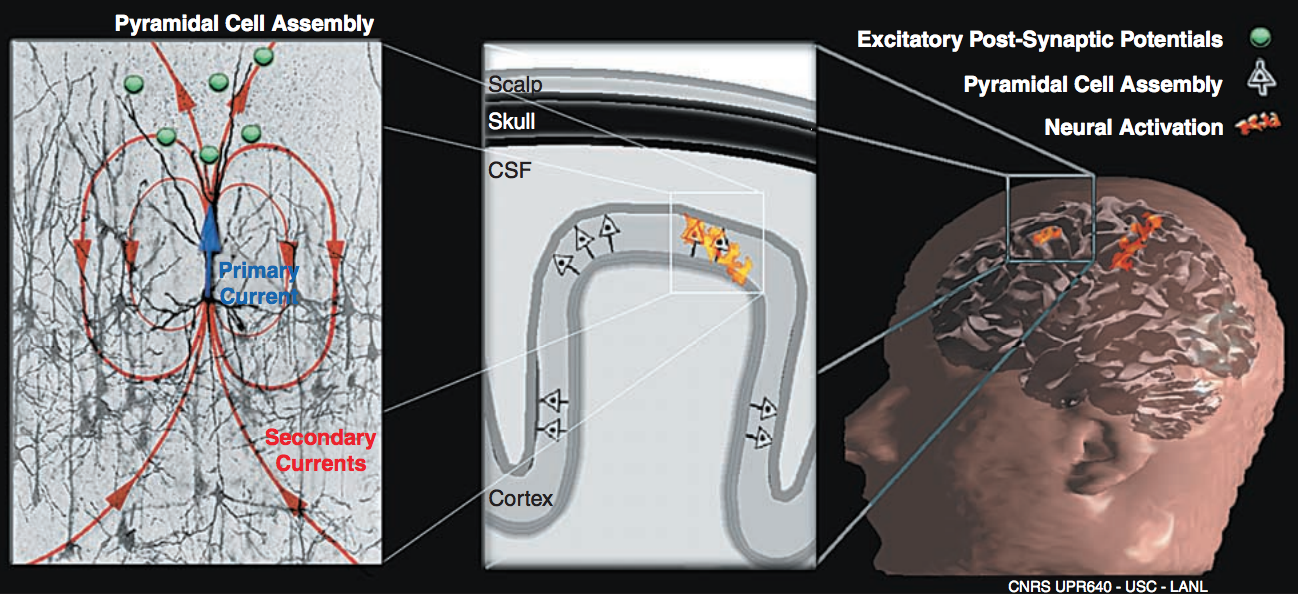
\includegraphics[width=0.95\textwidth]{background/network_cortical_neural_cells}
    \caption{Networks of cortical neural cell assemblies are the main generators of MEG/EEG signals. Left: Excitatory postsynaptic potentials (EPSPs) are generated at the apical dendritic tree of a cortical pyramidal cell and trigger the generation of a current that flows through the volume conductor from the non-excited membrane of the soma and basal dendrites to the apical dendritic tree sustaining the EPSPs. Center:  Large cortical pyramidal nerve cells are organized in macro-assemblies with their dendrites normally oriented to the local cortical surface. This spatial arrangement
and the simultaneous activation of a large population of these cells contribute to the spatio-temporal superposition of the elemental activity of every cell, resulting in a current flow that generates detectable EEG and MEG signals. Right: Functional networks made of these cortical cell assemblies and distributed at possibly mutliple brain locations are thus the putative main generators of MEG and EEG signals. Origin of this image is~\cite{baillet2001electromagnetic}
    }
    \label{fig:network_cortical_neural_cells}
\end{figure}

MEG and EEG are non-invasive functional imaging techniques for analyzing neural activity on a macroscopic scale. In contrast to indirect neuroimaging modalities, MEG and EEG signals derive from the net effect of ionic currents flowing in the dendrites of neurons during synaptic transmission. In accordance with Maxwell's equations, any electrical current will produce a magnetic field, and it is this field that is measured. The measurement principle of MEG and EEG is illustrated in Figure~\ref{fig:meg_eeg_principle}.\\

The neuronal activity captured by MEG is not, as perhaps expected, generated by the (too brief) axonal action potentials of pyramidal cells, but rather by the net contributions of excitatory and inhibitory dendritic postsynaptic potentials. This current flow through the apical dendrites (represented as a ‘dipole’) generates a magnetic field that projects radially; thus, MEG excels at detecting dipoles arranged in a tangential orientation to the skull. Fortunately, the extensively folded sulci of the human cortex promote that orientation for the majority of cortical microcolumns. However, MEG is less sensitive to deeper (including subcortical) sources, as magnetic field change decreases rapidly with distance.\\

\begin{figure}
	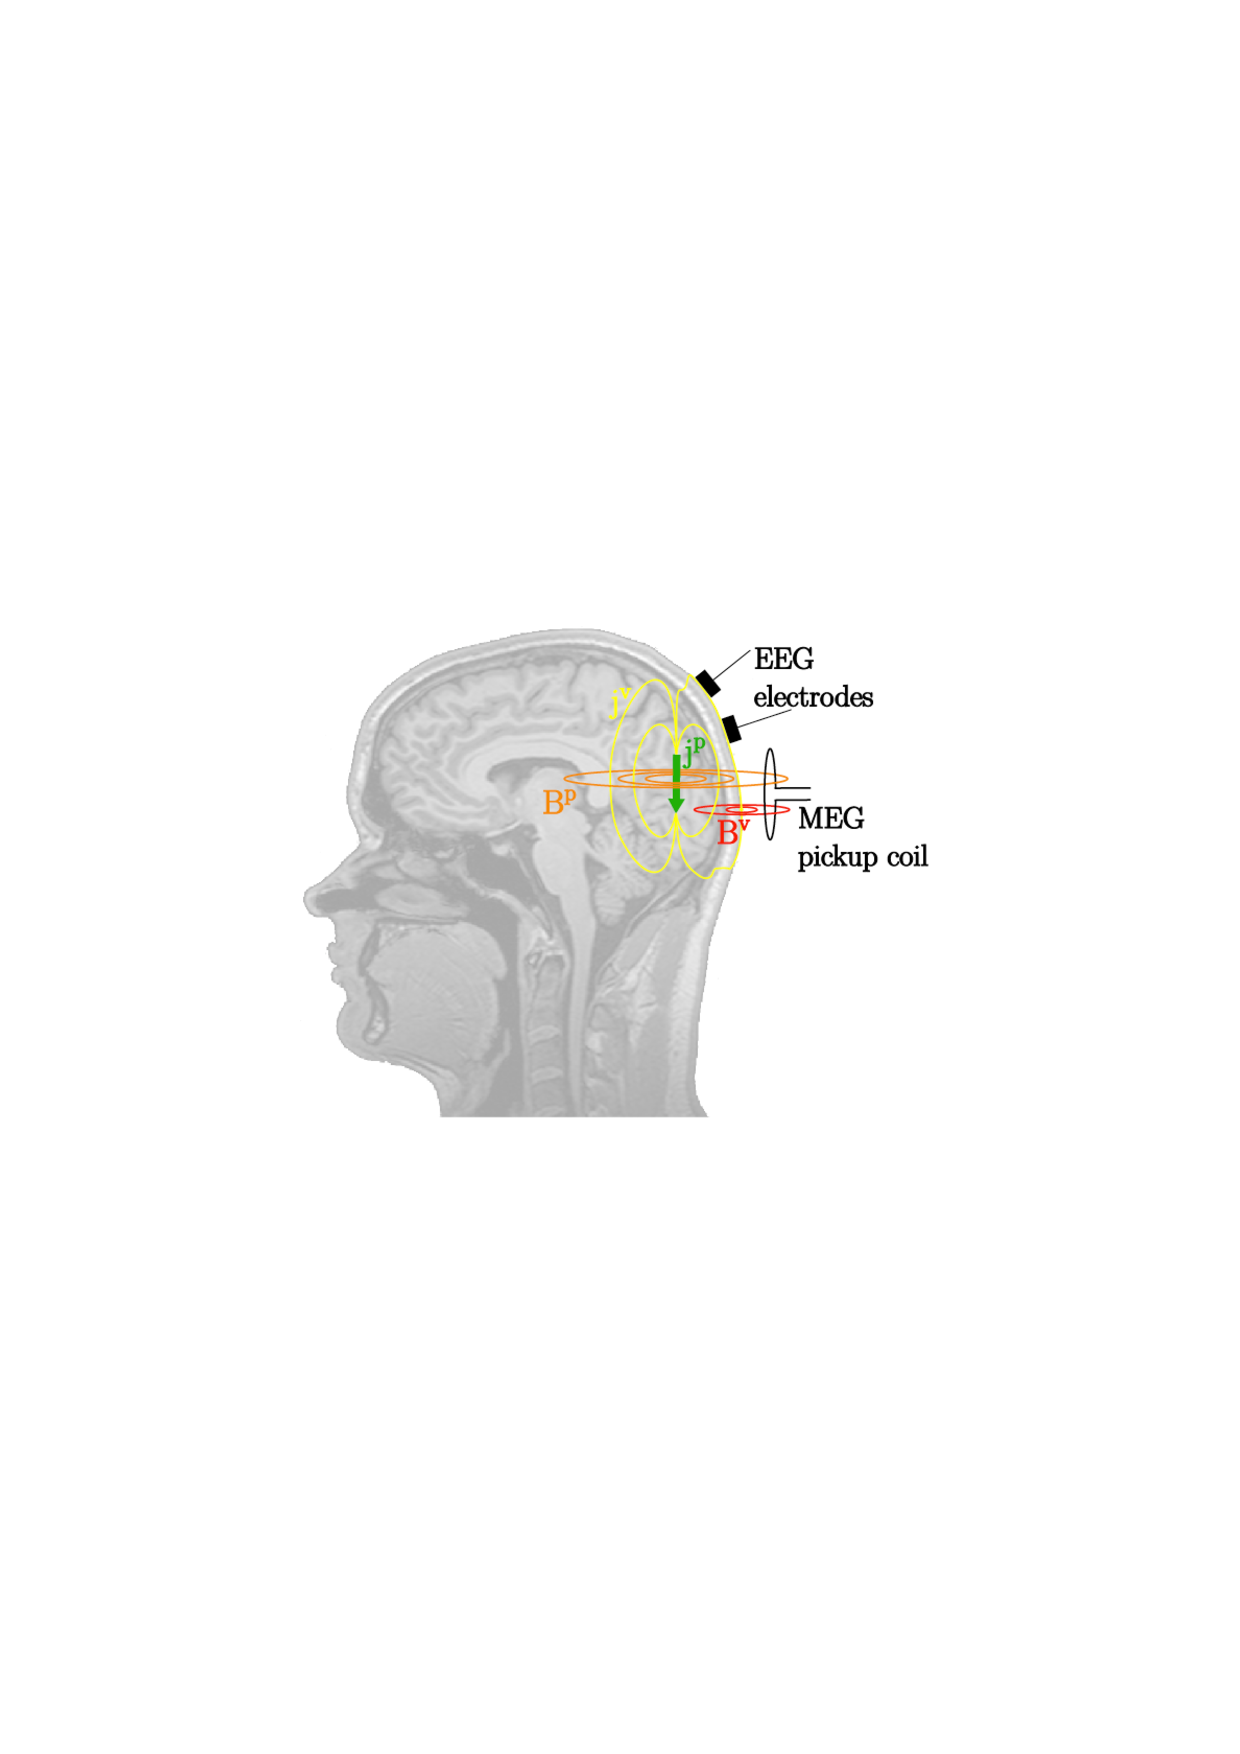
\includegraphics[trim={1cm 10cm 2cm 10cm},width=0.95\textwidth]{background/meg_eeg_principle}
    \caption{Simplified model of the measuring principle of MEG and EEG. The EEG measures the difference of the electric potential between the EEG electrode and a reference due to volume currents generated by primary currents in the brain. The
MEG captures the magnetic field generated by both primary and volume currents.
    }
    \label{fig:meg_eeg_principle}
\end{figure}

In 1969, the journey to understand the electrical potentials of the brain took an interesting and fruitful detour when David Cohen, a physicist working at MIT, became the first to confidently measure the incredibly tiny magnetic fields produced by the heart's electrical signals. To do this, he constructed a shielded room, blocking interference from the overwhelming magnetic fields generated by earth itself and by other electrical devices in the vicinity, effectively closing the door on a cacophony of voices to carefully listen to a slight whisper. His shielding technique became central to the advent of magnetoencephalography (MEG), which measures the yet even quieter magnetic fields generated by the brain's electrical activity.\\

This approach to record the brain's magnetic fields, rather than the electrical potentials themselves, was advanced even further by James Zimmerman and others working at the Ford Motor Company, where they developed the SQUID, a superconducting quantum interference device. A SQUID is an extremely sensitive magnetometer, operating on the principles of quantum physics, which is able to detect precisely those very tiny magnetic fields produced by the brain. To appreciate the contributions of magnetic shielding and SQUIDs to magnetoencephalography, consider that the earth's magnetic field, the one acting on your compass needle, is at least 200 million times the strength of the fields generated by your brain trying to read that very same compass.\\

In the other hand, the EEG measures the electric potential difference between the EEG electrode and a reference on the scalp associated with primary currents in the brain. These electric potential differences, which are in the range of a few microvolts, are recorded using amplifiers with high open-loop gain, common-mode rejection ratio, and input impedance. The first human EEG recording was done by Hans Berger in 1924.\\

MEG and EEG can be recorded simultaneously and reveal complementary properties of the electrical fields. Although the signals of EEG and MEG are generated by the same sources (electrical currents in the brain), they are both sensitive to different aspects of these sources. This could be compared to viewing the shadows of the same object from two different angles, combining the two recordings usually yields to better source estimation~\cite{malmivuo2012comparison,sharon2007advantage,aydin2015combined}.

%--------- Forward model -------------------------------------------------------------------
\section{The forward model}
The bioelectromagnetic forward problem describes the relationship between a given neural activity in the brain and the observable MEG and EEG signals. We assume the electric current (denoted by $\vec{j}_t(\vec{r})$) at any position (denoted by $\vec{r}$ in the head is known at arbitrary time $t$. The magnetic field or the sclap voltage detected by one sensor can be modeled as an integration or a linearly weighted combination of the currents at all positions, using Maxwell's equations under a reasonable head model that describes the shape, the electrical conductivity and the permeability of various tissues~\cite{hamalainen1993magnetoencephalography,mosher1999eeg}.

\subsection*{Maxwell's equations}
We consider the head as a finite three dimensional volume conductor, and non magnetic. The quasi-static approximation of Maxwell's equations are a set of partial differential equations forming the foundation of classical electromagnetism. We denote by $\mathbf{E}$ the electric field, $\mathbf{B}$ the magnetic field, $\mathbf{J}$ the current density, and $\rho$ the charge density.

\begin{center}
$\left\{
\begin{array}{l}
  \nabla . \mathbf{E} = \frac{\rho}{\epsilon} \\
  \nabla \times \mathbf{E} = \frac{-\partial \mathbf{B}}{\partial t} \\
  \nabla \cdot \mathbf{B} = 0 \\
  \nabla \times \mathbf{B} = \mu_0 (\mathbf{J} + \epsilon\frac{\partial \mathbf{E}}{\partial t})
\end{array}
\right.$
\end{center}

For the biological signals of interest in MEG/EEG, the time-derivatives of the associated electric and magnetic fields are sufficiently small that they can be ignored in Maxwell’s equations. Recent discussions and details of this quasi-static approximation can be found in\cite{hamalainen1993magnetoencephalography,tripp1983physical,heller1992brain}.\\

\subsection*{Spherical head models}
A very common approximation in the forward modeling consists in assuming that the head is a set of nested concentric spheres, each corresponding to a layer with homogeneous and isotropic conductivity. Typically, the head is represented by three to five regions, \textit{e.g.}, scalp, skull, cerebrospinal fluid, gray matter, and white matter, and that the conductivity is constant and isotropic within these regions. The gradient of the conductivity is, therefore, zero except at the surfaces between regions. Computable analytic solutions exist for both MEG and EEG forward problem.\\

A very practical formulation of the EEG and MEG field kernels has been presented by Mosher~\cite{mosher1999eeg}, that only requires vectors expressed in their Cartesian form. For MEG, since the magnetic permeability does not change across layers (and does not change much from the vacuum) and no currents exist outside the head (where the sensors are located), the full magnetic field outside a set of concentric spheres can be calculated without explicit consideration of the volume currents. Therefore, the MEG spherical model does not require specifying (or assuming) the number of and the radius ratios between the spherical layers.\\

For EEG, the number and radii of the spherical layers are to be specified. Nonetheless, previous empirical work on closed-form approximations by Berg and Scherg~\cite{berg1994fast} and related theoretical studies by Zhang~\cite{zhang1995fast} have gathered a valid and convenient method for approximating an EEG field kernel from a multi-layer spherical model as the weighted sum of three kernels from a single-layer spherical model applied to a modified source configurations. The optimal values of the "Berg parameters" (Eccentricity and Magnitude) in this approximation depend on the layer radii and conductivities.

\subsection*{Realistic head models}
A more realistic head model requires that the real geometry and conductivity of the head layers be taken into account as much as possible. For real (non-spherical) geometry and conductivity fields, numerical solutions for the Maxwell equations are to be computed.\\
Assuming a piecewise constant distribution of the conductivity field, approximate, yet efficient and accurate, numeric solutions can be obtained for a realistically shaped head model using the so called Boundary Element Method (BEM). For BEM solutions, an MRI-based simplified description of the geometry is needed for computing the lead fields, and this can be provided in terms of (strictly) nested and closed surfaces corresponding to the boundaries separating the main tissue compartments (also called layers).
In practice, BEM solutions will only require to set a few conductivity parameters (one per tissue), and to specify a few triangular meshes, as can be obtained, \textit{e.g.}, with 3D volume segmentation tools from anatomical MRI data (VMR), each representing a separate interface between layers. \\
\textbf{XXX: See MNE doc}.

% http://leonidzhukov.net/content/eeg_meg_physics/node1.html
% http://www.brainvoyager.com/bvqx/doc/UsersGuide/EMEGSuite/EEGAndMEGForwardModels.html

%--------- MEEG inverse problem ------------------------------------------------------------
\section{M/EEG Inverse problem}
\emph{\textbf{Notation}}
All matrices and vectors are written in bold letters. Matrices, such as $\mathbf{A}$, are written in upper case, whereas vectors, such as $\mathbf{b}$, are in lower case. A matrix $\mathbf{A} \in \RR^{M\times N}$ has $M$ rows and $N$ columns. Its transpose is denoted $\mathbf{A}^\mathbf{T}$, and its Hermitian conjugate $\mathbf{A}^\mathcal{H}$. $\mathbf{A}[i,:]$ and $\mathbf{A}[:,j]$ correspond to the $i^{th}$ row the $j^{th}$ column respectively, and $\mathbf{A}[i,j]$ to the element in the $i^{th}$ row and $j^{th}$ column of $\mathbf{A}$.
$\|\mathbf{A}\|_{Fro}$ stands for the Frobenius norm. Matrix $\mathbf{I}$ stands for the identity matrix.

\subsection{Parametric models: \textit{dipole fitting}} \label{section_dipfit}
The goal of inverse methods is to estimate the location, orientation and the strengths of the current sources that generate the M/EEG measurements.
The dipole fitting approaches \cite{scherg1985two} assume that the measured data have been produced by a small number of active brain regions that can each be modeled using an equivalent current dipole. These algorithms minimize a data-fit cost function such as the Frobenius norm of the residual, and they estimate five non-linear parameters per dipole: the 3D $(x,y,z)$ position, and the two angles to define the dipole orientation. The main limitation of these methods is that they cannot be used when complex cognitive tasks are performed. This is due to the fact that the optimization problem to be solved is not linear, which implies that it gets easily trapped in local minima as soon as one tries to localize more than two dipoles. Furthermore, the number of dipoles to be estimated is not known and then needs to be set in advance. 

\subsection{Scanning methods: \textit{beamforming \& MUSIC}}
Scanning methods, \textit{a.k.a.} beamforming, use a discrete grid to search for optimal dipole positions throughout the source space. An estimator of the contribution of each source location to the data can be derived either via spatial filtering or signal classification settings. The simplest spatial filter is \textit{a matched filter}, but the most common one is the linearly constrained minimum variance (LCMV) beamformer \cite{van1997localization}.
%and multiple signal classification (MUSIC) methods and their variants.\\
LCMV performs a spatial filtering on data to discriminate between signals originating from a location of interest and those coming from elsewhere, and limits the influence of the noise. In practice, it implies that the measurement matrix is multiplied by a weighting matrix. The weighting matrix should pass signals coming from the location of interest, while attenuating signals from elsewhere. LCMV determines the weighting matrix by minimizing the output power of a filter under a constraint that its gain (forward operator) is unity at the location of interest. An attractive feature of beamforming is that it does not require any assumptions on the number of the underlying sources, however it makes the strong assumption that the activations of the different sources are uncorrelated, which is not the case. An alternative to LCMV which integrates some information related to the experimental paradigms is called Synthetic Aperture Magnetometry (SAM) \cite{vrba2001signal}. Beamforming can also be applied in the frequency domain using the dynamic imaging of coherent sources (DICS) \cite{gross2001dynamic}.
%The difference between beamformers is the constraint for estimating the weighting matrix. LCMV determines the weighting matrix by minimizing the output power of a filter under a constraint that its gain is unity at the location of interest. The limitation of this approach is that signal cancellation may occur, when different sources are correlated (Baillet et al. 2001). Another beamformer often used is Synthetic Aperture Magnetometry (SAM) (Vrba and Robinson, 2001).\\

Alternatives to beamformers are methods based on signal classification using subspace decomposition. The MUltiple SIgnal Classification (MUSIC) is a widely known signal processing technique that was first applied to EEG data by \textit{Mosher} \cite{mosher1992multiple}. The primary assumptions for this method are that the dipolar time series are mutually linearly independent. 
MUSIC is based on a singular value decomposition (SVD) of the measurement data, which results in orthogonal basis vectors and singular values. Any true source localization will have a lead field (forward) vector which lies in the signal subspace computed with the SVD. MUSIC scans the brain space for source locations that satisfy this condition. The lead field vector at every candidate dipole location is systematically projected on the signal subspace. The dipole source locations with the largest projections on the signal subspace are the active sources \cite{mosher1992multiple,mosher1999source}. However, MUSIC suffers from some problems. First, when the noise present in the data is correlated across channels, MUSIC can produce larger errors in the dipole localization than would have been observed with uncorrelated noise of the same power. Another problem is the detection of multiple MUSIC peaks in a 3D space of the head, each of which may correspond to a different ECD. A related problem is to determine which peaks are truly indicative of a dipolar source rather than a local minimum in the error function \cite{mosher1999source}.

The later problem is solved in an extended version of MUSIC, Recursively Applied and Projected (RAP)-MUSIC, by recursive estimation of multiple sources \cite{mosher1997source,mosher1999source}. In other words, it consists in applying MUSIC successively after removing the contribution of the previously identified sources. Such as matching pursuit algorithms are used for sparse signal decomposition over dictionary of atoms \cite{mallat1993matching}, the RAP-MUSIC method adopts a greedy strategy to select the relevant dipoles in a dictionary of sources. The implementation of RAP-MUSIC and its comparison with another solver was the first contribution of this thesis \cite{irMxNE}.
%Recently, an alternative method was developed called FINES (Xu, et al., 2004). This method is able to localize closely spaced correlated sources.

\subsection{Probabilistic modeling: \textit{distributed sources \& Bayesian approaches}} \label{section_distributed}
Distributed source localization estimates the amplitudes of a dense set of dipoles distributed at fixed locations within the head surface/volume. These methods are based on reconstruction of the brain electric activity in each point of a 3D grid of solution points, the number of points being much larger that the number of electrodes on the scalp. Each solution point is considered as possible location of a current source, thus there is no a priori assumption on the number of dipoles in the brain.
When orientations are fixed and only the amplitudes of the sources are estimated, the forward problem results in a regression formulation.%in Eq.\ref{eq_linmeeg}.

We present in the second part of this chapter how the M/EEG inverse problem with distributed source models leads to a regularized regression problem. The widely known \textit{Minimum Norm Estimate} (MNE) minimizes the $\ell_2$-norm \cite{hamalainen1994interpreting}. %The standard MNE is given in Eq.\ref{eq_thikonov}.
MNE has been very attractive due to the fact that the inverse solution is given by a simple matrix multiplication ($\ell_2$-based methods). However, the choice of the $\lambda$ parameter as the trade-off between data fit and regularization is sometimes tricky, because it depends on the data since $\lambda$ is related to the noise level present in the measurement. $\lambda$ is most of the time chosen with a cross-validation strategy to find the optimal value.

When applying a minimum-norm estimate, all the sources are penalized equivalently. This approach introduces bias over source, which are farther from the sensors than the others, \textit{i.e.} sources which are close to the sensors have a higher forward field. This implies that the effect on the sensors of a small activation is big; those sources are called superficial sources. This results in the introduction of a Weighted Minimum Norm (WMN) estimate \cite{lin2006assessing}, which downweights the dipoles in the head that are closer to the surface. However, the current predicted inside the head is very blurred. Therefore, an alternative method has been developed called FOCUSS (FOCal Underdetermined System Solution) \cite{gorodnitsky1995neuromagnetic}. This method changes the weights at each iteration to overcome the problem. The limitation of this method is that it does not take any biophysiological information into account, and might get stuck in local minima.

Another method for the M/EEG inverse problem is Low Resolution brain Electromgnetic Tomography (LORETA) \cite{pascual1994low}. This method tries to find the smoothest possible solution, however it generally provides very blurred (over-smoothed) solutions.

Another idea to investigate the M/EEG source localization was the use of noise normalized methods. Those methods like dSPM \cite{dale2000dynamic} and sLORETA \cite{pascual2002standardized}, aim to represent on the cortex not the activity itself, but a \textit{dimensionless} statistical quantity. The reason why dSPM has been widely used in the MEG community is the fact that using this statistical quantity reduces the bias towards the superficial sources and makes all kind of thresholding easy on the source estimate.

The methods cited in the previous paragraphs consider spatial smoothness prior on the inverse problem. However, they do not take the time dependence of the M/EEG data into account. Also they are dense models, which do not fit the assumption that only a few focal brain regions are involved in a specific cognitive task. MNE or dSPM for example will both have nonzero sources for every time instant.
For this aim, several methods favoring sparse focal source configurations have been proposed: Selective minimum-norm \cite{matsuura1995selective}, Sparse Bayesian Learning (SBL) \cite{wipf2006bayesian}, Spatio-Temporal TOmographic NonNegative Independent Component Analysis (STTONNICA) \cite{valdes2009eeg}, mixed-norms \cite{ou2009distributed}, Champagne \cite{owen2012performance}, hierarchical Bayesian inference  \cite{lucka2012hierarchical}, or the Mixed-Norm estimates (MxNE) \cite{gramfort2012mixed}. Those methods are called spatio-temporal because they work in a predefined time window, however they completely ignore the temporal correlation. This can be verified by shifting the columns of the source estimate, it will have no effect on the source estimate itself. To introduce a "true" spatio-temporal constraint in the model, \cite{zhang2011sparse,zhang2011iterative} incorporated the temporal correlation to improve the source estimates, \cite{gramfort2013time} reused the MxNE in the time-frequency domain in the Time-Frequency Mixed-Norm Estimate (TF-MxNE), and \cite{castano2015solving} introduces Spatio-Temporal Unifying Tomography (STOUT).

Although these spatio-temporal methods are improving the M/EEG source reconstruction, they are based on convex penalties. This allows fast algorithms with guaranteed global convergence. However, the resulting source estimates are biased in amplitude and often suboptimal in terms of support recovery, \textit{i.e.}, active sources \cite{candes2008enhancing}. As shown \textit{e.g.} in the field of compressed sensing, promoting sparsity by applying non-convex penalties, such as logarithmic or  $\ell_p$-quasinorm penalties with $0<p<1$, improves support reconstruction in terms of feature selection, amplitude bias, and stability \cite{candes2008enhancing,chartrand2007exact,saab2008stable}. Several approaches for solving the resulting non-convex optimization problem have been proposed including iterative reweighting $\ell_1$ optimization \cite{candes2008enhancing}. \cite{strohmeier2014iterative} used an iterative reweighted approach to solve the composite non-convex penalty in the time-frequency domain.

%\textbf{Local autoregressive average (LAURA)}\\
%\textbf{EPIFOCUS}\\

%\subsection{Minimum norm solutions and its \textit{sparse} variants}
%\subsection{Other methods}
%\textbf{Bayesian method}\\
%\textbf{ELECTRA}\\

%https://books.google.fr/books?id=s1VfR1T3P08C&pg=PA85&lpg=PA85&dq=inverse+problem+meg+book+bird+image&source=bl&ots=dZ-XzI5x7M&sig=1TVAsYPk1t4AD_XzyeGqduIp97s&hl=en&sa=X&ved=0ahUKEwikzKrVi6_MAhWCUBQKHRqQAwwQ6AEIIzAB#v=onepage&q&f=false

%http://www.fil.ion.ucl.ac.uk/~wpenny/publications/spm-book/steeg.pdf

%https://books.google.fr/books?id=YLyGmfVuBsIC&pg=PA192&lpg=PA192&dq=inverse+problem+meg+book&source=bl&ots=q2QE3dxz__&sig=OElFKShtnznrpaCeLHZMbTAOBmw&hl=en&sa=X&ved=0ahUKEwj95bm9iq_MAhWCvxQKHWCeA3MQ6AEIWjAI#v=onepage&q=inverse%20problem%20meg%20book&f=false

\subsection{Conclusion}
This part has presented an overview on the state of the art of the MEG and EEG inverse solvers. Although multiple solvers have been provided, this list is definitely not exhaustive.
We have kept at the end the distributed solvers which are the main interest of this thesis. Here, we will model the problem as a regularized regression with sparse priors. In the next part of the chapter, we discuss all aspects of linear regression, different penalization terms, especially the ones promoting sparsity, and the algorithms to solve those optimization problems.

%-----------------Time-Frequency------------------------------------------------------------
\section{Time-Frequency representation}
\label{section:TF}
% http://www.dafx.ca/slides/keynote1.pdf
In signal processing, time-frequency analysis comprises those techniques that study a signal in both time and frequency domains simultaneously, using various time-frequency representations (TFR). During the last decades, signal processing community has provided many new techniques for expanding signals into "elementary" waveforms, such as wavelet bases, modified discrete cosine transform (MDCT), short time Fourier transform (STFT), Gabor wavelets (frames), etc. More often, the key issue is to obtain a sparse representation of the signal, when it is better defined in the frequency domain than the time domain. For example, a sine wave is sparsely represented in the Fourier domain, not in the time domain.\\

A signal representation is sparse when most information is concentrated in a small amount of data or coefficients. Several applications make use of the sparse TFR as denoising because the noise is not sparse, source separation, signal modeling, etc. To decompose a signal into a linear combination of "elementary" waveforms $\psi_{\lambda}$, often generated using simple rules:
\begin{equation}\label{eq_signal_decomp}
x(t) = \sum_i\alpha_i\psi_i(t)
\end{equation}
with $\alpha_i$ the coefficients, and $\psi_i$ the waveforms. See \cite{mallat2008wavelet,hlawatsch1992linear,wickerhauser1994adapted} for detailed examples of signal representations.\\

\subsection{Modified Discrete Cosine Transform: MDCT}
The mathematically simplest situation for signal decomposition is orthonormal bases. The waveform system $\mathcal{W}=\{\psi_i, i \in\Lambda\}$ is an orthonormal basis of the signal space (inner product space, or Hilbert space) $\mathcal{H}$ is:
\begin{itemize}
\item The atoms are mutually orthogonal and normalized: $\langle\psi_i,\psi_j\rangle = 0$ and $\|\psi_i\|=1$
\item They form a complete set of $\mathcal{H}$: if the signal $x\in\mathcal{H}$ is such that $\langle x,\psi_i\rangle=0$ for all $i\in\Lambda$, then $x=0$.
\end{itemize}
Then, any signal can be written in a unique way as in Equation~\ref{eq_signal_decomp} with $\alpha_i=\langle x,\psi_i\rangle$.\\

MDCT basis vectors are shift variant, it does not conserve the energy \& MDCT coefficients are real valued. They cannot be easily interpreted in terms of magnitude and phase, all these reasons say that MDCT is purely appropriate for spectral analysis and signal manipulation in the TF domain.

\subsection{Gabor dictionaries}
Given a signal observed over a time interval, its conventional Fourier transform computes the frequency content but loses the time information. To analyze the evolution of the spectrum with time and hence the non-stationarity of the signal, Gabor introduced windowed Fourier atoms which correspond to a short-time Fourier transform (STFT) with a Gaussian window. In practice, for numerical computation, a challenge is to properly discretize the continuous STFT. The discrete STFT with a Gaussian window is also known as the discrete Gabor Transform \cite{gabor1946theory}.

The setting we consider is the finite-dimensional one. Let $\mathbf{g}\in \RR^{T}$ be a "mother" analysis window. Let $f_0\in \mathbb{N}$ and $k_0\in \mathbb{N}$ be the frequency and time sampling rates in the time-frequency plane generated by the STFT, respectively. The family of the translations and modulations of the mother window generates a family of Gabor atoms $(\mathbf{\phi}_{mf})_{mf}$ forming the dictionary $\mathbf{\Phi}\in \mathbb{C}^{T\times K}$, where $K$ denotes the number of atoms. The atoms can be written as:
\begin{equation} \label{eq_gabor_atoms}
	\mathbf{\phi}_{mf}[n] = \mathbf{g}[n-mk_0]e^{\frac{i2\pi f_0 fn}{T}}, m\in \{0,\dots ,\frac{T}{k_0}-1\}, f\in \{0,\dots ,\frac{T}{f_0}-1\}.
\end{equation}
If the product $f_0k_0$ is small enough, \textit{i.e.}, the time-frequency plane is sufficiently sampled, the family $(\mathbf{\phi}_{mf})_{mf}$ is a frame of $\RR^T$, \textit{i.e.}, one can recover any signal $\mathbf{x}\in \RR^T$ from its Gabor coefficients $(\langle \mathbf{x}, \mathbf{\phi}_{mf}\rangle)=\mathbf{\Phi}^{\mathcal{H}}\mathbf{x}$. More precisely, there exists two constants $A, B > 0$ such that:
\begin{equation} \label{eq_frame}
	A\|x\|_2^2 \leq \sum_{m,f}|\langle \mathbf{x}, \mathbf{\phi}_{mf}\rangle|^2\leq B\|x\|_2^2   
\end{equation}
When $A=B$, the frame is \textit{tight}. When the vectors $\mathbf{\phi}_{mf}$ are normalized, the frame is an orthogonal basis if and only if $A=B=1$. The Balian-Low theorem says that it is impossible to construct a Gabor frame which is a basis. Consequently, a Gabor transform is redundant or overcomplete and there exists an infinite number of ways to reconstruct $\mathtt{x}$ from a given family of Gabor atoms. In the following, the considered $\mathbf{\Phi}$ dictionaries are tight frames.

The canonical reconstruction of $\mathbf{x}$ from its Gabor coefficients requires a canonical dual window, denoted by $\mathbf{\tilde{g}}$. Following \ref{eq_gabor_atoms} to define $(\tilde{\mathbf{\phi}}_{mf})_{mf}$ we have:
\begin{equation} \label{eq_TF_recons}
	\mathbf{x}=\sum_{m,f}\langle\mathbf{x}, \mathbf{\phi}_{mf}\rangle\tilde{\mathbf{\phi}}_{mf}=\mathbf{\Phi}^{\mathcal{H}}\mathbf{x\tilde{\Phi}}=\tilde{\mathbf{\Phi}}^{\mathcal{H}}\mathbf{x\Phi},
\end{equation}
where $\tilde{\mathbf{\Phi}}$ is the Gabor dictionary formed with the dual windows. If the frame is tight, then we have $\tilde{\mathbf{g}}=\mathbf{g}$, and more particularly we have $\mathbf{\Phi\Phi}^{\mathcal{H}}=\|\mathbf{\Phi\Phi}^{\mathcal{H}}\|\mathbf{I}$. The representation being redundant, for any $\mathbf{x}\in\RR^T$ one can find a set of coefficients $z_{mf}$ such that $\mathbf{x}=\sum_{m,f}z_{mf}\mathbf{\phi}_{mf}$, while the $z_{mf}$ verify some suitable properties dictated by the application. For example, it is particularly interesting for MEG/EEG to find a sparse representation of the signal. Indeed, a scalogram, sometimes simply called TF transform of the data in the MEG literature, generally exhibits a few peaks localized in the time-frequency domain. In other words, MEG/EEG signals can be expressed as linear combinations of a few oscillatory atoms. In order to demonstrate this, Fig. \ref{fig:stft} shows the STFT of a single signal from a MEG channel from a somatosensory experiment, the same STFT restricted to the 50 largest coefficients (approximately only 10\% of the coefficients), and the signal reconstructed with only these coefficients compared to the original signal. We observe that the original signal can be very well approximated by only a few coefficients, \textit{i.e.}, a few Gabor atoms.

\begin{figure}
\centering
	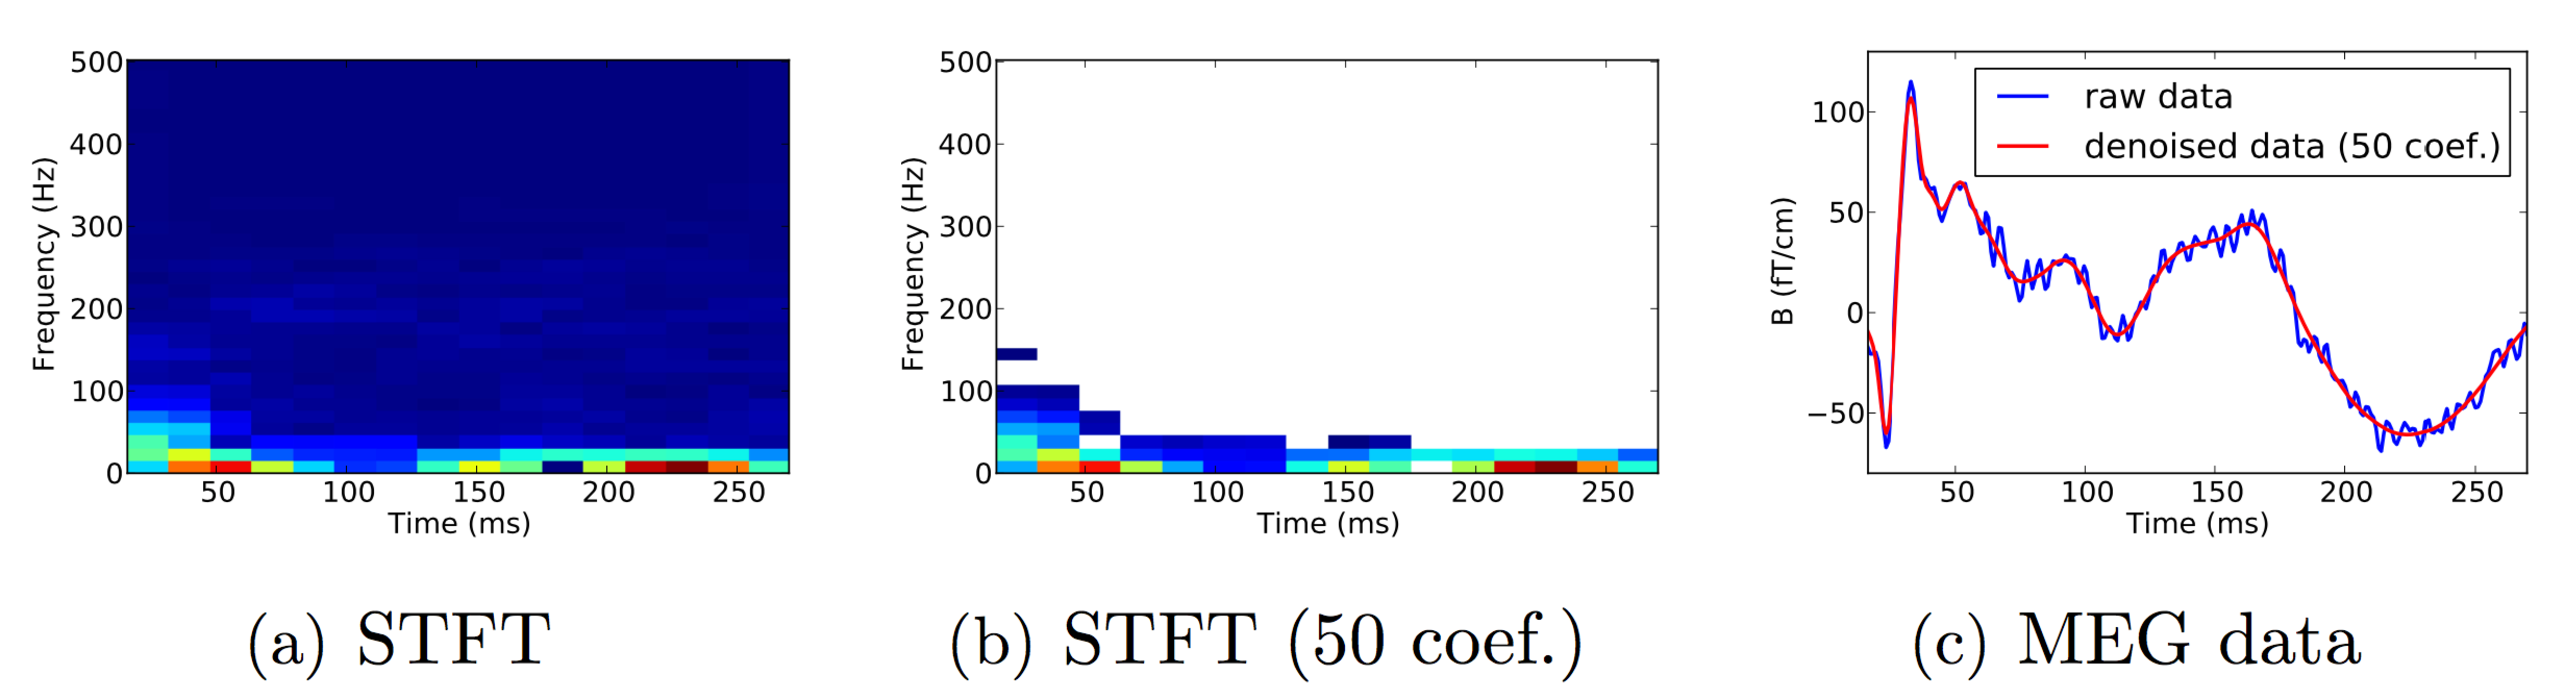
\includegraphics[width=\textwidth]{stft}
    \caption{a) Short-time Fourier transform (STFT) of a single channel MEG signal sampled at 1000Hz showing the sparse nature of the transformation (window size 64 time points and time shift $k_0=16$ samples). b) STFT restricted to the 50 largest coefficients. c) Data and the reconstructed data using only the 50 largest coefficients.}
	\label{fig:stft}
\end{figure}

In practice, the Gabor coefficients are computed using the Fast Fourier Transform (FFT) and not by a multiplication by a $\mathbf{\Phi}$ matrix as suggested above. Such operations can be efficiently implemented as in the LTFAT toolbox\footnote{http://ltfat.sourceforge.net} \cite{sondergaard2012linear}. Another practical concern to keep in mind is the trade-off between the size of the window $\mathbf{g}$ and the time shift $k_0$. A long window will have a good frequency resolution and a limited time resolution. The time resolution can be improved with a small time shift, leading however to a larger computational cost, both in time and memory. Finally as any computation done with an FFT, the STFT implementations assume circular boundary conditions for the signal. To take this into account and avoid edge artifacts, the signal has to be windowed, \textit{e.g.}, using a Hann window.\\

For more details about Gabor dictionaries, please refer to \cite{daubechies1992ten}.

\subsection{Conclusion}

This last part briefly introduced some important properties of time-frequency representation. It presented MDCT and Gabor dictionaries. It mainly explained the advantage of using the tight Gabor frames concept. Short Term Fourier Transform (STFT) or Gabor frames are time invariant in contrast of MDCT. Chapter~\ref{chapter:multiscale} will model the inverse problem in the time-frequency domain, which is based on the construction of Gabor frames. 

%-----------------Optimization--------------------------------------------------------------
\section{Optimization}
Due to the fact that the MEG/EEG sensors are linear combinations of the electromagnetic fields produced by all current sources, the linear forward operator, called \textit{gain matrix}, or the \textit{mixing matrix}, predicts the MEG/EEG measurements. Here we introduce the linear regression on what is based the formulation of the M/EEG inverse problem in this thesis.

\subsection{Linear model and regression}
%\textbf{XXX: intro to convexity...}
In compressed sensing, linear regression consists of modeling the linear relationship between an observation $y$ and an explanatory variable $\mathbf{s}=[s[1],\dots ,s[m]]^T$, this relationship results from the existence of $\mathbf{x}\in\RR^m$ such that:
\begin{equation} \label{eq_linreg}
	\langle\mathbf{s}, \mathbf{x}\rangle = y
\end{equation}
This linear model is verified for a set of observations coming from the same event, \textit{i.e.}, the linear combination defined by $\mathbf{x}$ is the same for all (variable, observation) couples originating from the same event: $(\mathbf{s}^i, y[i])\in\RR^m\times\RR$ with $i\in [1,\dots ,n]$. We can note $[y[1], \dots ,y[n]]^T=\mathbf{y}\in\RR^n$ and $[\mathbf{s}^1,\dots ,\mathbf{s}^n]=\mathbf{D}\in\RR^{m\times n}$. If all couples $\{(\mathbf{s}^i,y[i])\}_{i\in [1,\dots ,n]}$ verify exactly a linear model, then there exists a $\mathbf{x}\in\RR^m$ such that $\mathbf{Dx}=y$.

In a MEG/EEG application, the equivalent of $\mathbf{D}$ is the forward operator $\mathbf{G}$ which describes the linear relationship between the MEG/EEG measurements $\mathbf{M}\in\RR^{N\times T}$ ($N$ number of sensors, $T$ number of time instants) and the source activation $\mathbf{X}\in\RR^{S\times T}$ ($S$ is the number of source locations). The linear model then reads: $\mathbf{M} = \mathbf{GX}$ where $\mathbf{G}\in\RR^{N\times S}$ is the gain or the lead-field matrix (forward operator), a known instantaneous mixing matrix, which links source and sensor signals. 

In practice, the linear model is never exactly verified due to external noise. The aim of the linear regression is to additionally assume that an unobserved random variable, \textit{i.e.}, error term is added to the linear relationship between the M/EEG measurements $\mathbf{M}$ and the source activation $\mathbf{X}$. The regression model can then be written as:
\begin{equation} \label{eq_linmeeg}
	\mathbf{M} = \mathbf{GX} + \mathbf{E}
\end{equation}
where $\mathbf{E}$ is the measurement noise, which is assumed to be additive, white, and Gaussian, \mbox{$\mathbf{E}[:,j]\sim\mathcal{N}(0,\mathbf{I})$} for all $j$. This assumption is acceptable on the basis of a proper spatial whitening of the data using an estimate of the noise covariance \cite{engemann2015automated}.

Several methods exist to approximate the solution of the regression model, the most widely used is the least square (LS) approach \cite{legendre1805nouvelles}, which minimizes the sum of the squares of the errors or residuals as follows:
\begin{equation} \label{eq_ls}
	\mathbf{X^\star} = \argmin_{\mathbf{X}\in \RR^{S\times T}}\frac{1}{2} \|\mathbf{M}-\mathbf{GX}\|_{Fro}^2
\end{equation}
There exist other types of approaches like the least absolute deviations (LAD), also known as least absolute errors. Instead of minimizing the squares of the errors, LAD tries to minimize the sum of the absolute values of the errors/residuals. Its advantage over LS is that it is more robust to outliers in the data. However the LAD is not stable, \textit{i.e.}, a small modification of the observation $\mathbf{M}$ may result in a huge variation of the estimation of $\mathbf{X}$. Moreover it can have multiple solutions. This explains why the LS approach has been the standard one and also due to the fact that it has a closed-form solution.

\subsection{Regularization}

Regularization in general can be applied for different reasons. We have seen why the least squares is the standard approach in linear regression. However this approach has some drawbacks: \textit{overfitting} and the fact that the closed-form solution is computed using $\mathbf{G}^T\mathbf{G}$, which might not be invertible, giving rise to an infinitely many solutions. This requires to set regularization.\\

In general, the penalization term will be marked $\mathcal{P}(\mathbf{X})$ as in \ref{eq_reg} and it can take any dense or sparse form.
\begin{equation} \label{eq_reg}
	\mathbf{X}^\star = \argmin_{X\in\RR^{S\times T}}\frac{1}{2}\|\mathbf{M}-\mathbf{GX}\|_{Fro}^2 + \lambda\mathcal{P}(\mathbf{X})
\end{equation}
We can list the different regularization term $\mathcal{P}(\mathbf{X})$ as the one using: dense norms, convex sparse norms, non-convex sparse norms, and structured norms.

\subsubsection*{Dense norms}
Thikonov regularization \cite{tikhonov1977solutions} is the most commonly used, also known as rigde regression \cite{hoerl1970ridge}. It is part of dense norms as the estimated $\mathbf{X}^\star$ is dense, even if most of its values are almost zero. It reads:
\begin{equation} \label{eq_thikonov}
	\mathbf{X}^\star = \argmin_{X\in\RR^{S\times T}}\frac{1}{2}\|\mathbf{M}-\mathbf{GX}\|_{Fro}^2 + \lambda\|\mathbf{X}\|_2^2
\end{equation}

The first term of the minimization is called the data fit, and the second term penalizes the solution by keeping the values of $\mathbf{X}$ small. The penalization is controlled by the $\lambda>0$ parameter. The higher it is, the more penalized the regression is. An explicit solution of \ref{eq_thikonov} is given by $\mathbf{X}^\star = (\mathbf{G}^T\mathbf{G}+\lambda\mathbf{I})^{-1}\mathbf{G}^T\mathbf{M}$. 

In this thesis, we are interested in sparse regularization, which has more sense in the MEG/EEG application. Since a few focal regions in the brain are active during a cognitive task rather than the whole brain itself. Using sparse priors can enable us to penalize the solution for this aim.

\subsubsection*{Sparse norms: \textit{Convex norms}}
In general, let $\mathbf{y}\in\RR^n$ be a sparse vector, \textit{i.e.} which belongs to a vector subspace $S$, which has a much smaller dimension $n^\prime\ll n$. 
The intuitive measure of sparsity of a vector $\mathbf{y}$ is its pseudo-norm $\ell_0$, which is defined as: $\|\mathbf{y}\|_0\triangleq \#\{i=1,\dots ,n | y[i]\neq 0\}$. It denotes its number of coefficients which are different from 0. The optimization problem is then to find the subspace $S$ where the signal $\mathbf{y}$ lies.\\

Coming back to our application, we assume that the signals $\mathbf{M}$ obtained with M/EEG are linear combinations of a small number of sources in the brain. This implies that only few sources in $\mathbf{X}$ are active, \textit{i.e.}, $\mathbf{X}$ is sparse. However the minimization of \ref{eq_reg} with $\ell_0$-norm is not computationally tractable. This problem is difficult as we need to select the the number of sources. Furthermore, the $\ell_0$-norm is not convex \cite{natarajan1995sparse}.

Due to the above undesired properties, we need to consider a convex relaxation to the $\ell_0$-norm. The use of the least squares with the $\ell_1$-norm (i.e. $\mathcal{P}(\mathbf{X})=\|\mathbf{X}\|_1$ in \ref{eq_reg}) is the natural approximation, since it is the closest convex norm to the $\ell_0$-norm. The $\ell_1$-norm is known as \textit{lasso} in statistics \cite{tibshirani1996regression}, and as Basis Pursuit \cite{chen2001atomic} in signal processing literature.

\adjustwidth{1em}{0pt}
\subsubsection*{Lasso}
\begin{equation} \label{eq_lasso}
	\mathbf{X}^\star = \argmin_{\mathbf{X}\in\RR^{S\times T}}\frac{1}{2}\|\mathbf{M}-\mathbf{GX}\|_{Fro}^2 + \lambda\|\mathbf{X}\|_1
\end{equation}
\endadjustwidth
The convex approximation of the $\ell_0$-norm is convenient, as the method always converges to the optimal solution.

\subsubsection*{Sparser norms: \textit{Non-Convex norms}}
These convex approaches allow for fast algorithms with guaranteed global convergence. However, the resulting source estimates are biased in amplitude and often suboptimal in terms of support recovery~\cite{candes2008enhancing}, which is impaired by the high spatial correlation of the MEG/EEG forward model. As shown e.g. in the field of compressed sensing, promoting sparsity by applying non-convex penalties, such as logarithmic or $\ell_p$-quasinorm penalties with $0 < p < 1$, improves support reconstruction in terms of feature selection, amplitude bias, and stability~\cite{candes2008enhancing,chartrand2007exact,saab2008stable}. Figure~\ref{fig:norms} shows the geometric interpretation of different norms in the 1-dimensional space. The smaller the $p$, the more you approximate the exact definition of sparsity. 

\begin{figure}
\centering
	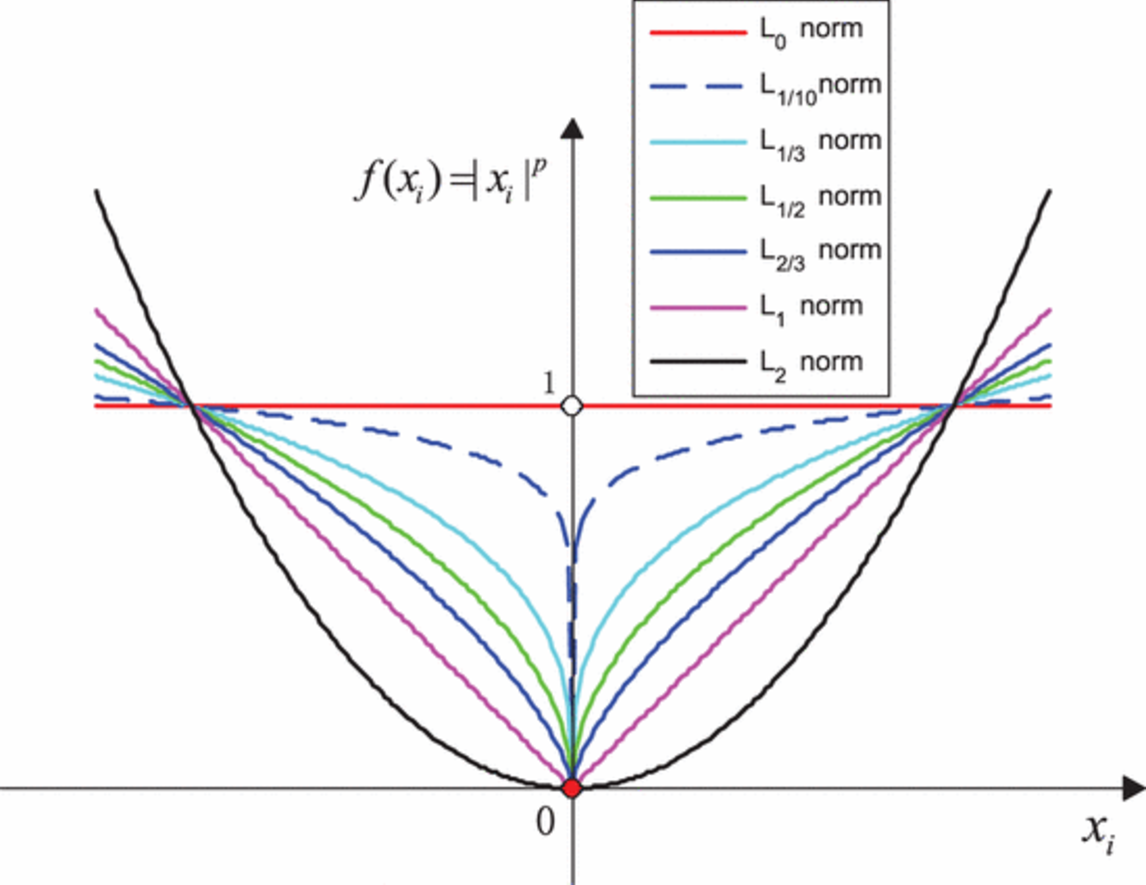
\includegraphics[width=0.6\textwidth]{norms}
    \caption{Geometric interpretation of the different norms in 1D space.}
	\label{fig:norms}
\end{figure}

We investigated the $\ell_{0.5}$-quasinorm as part of the regularization, written as:
\adjustwidth{1em}{0pt}
\subsubsection*{$\ell_{0.5}-quasinorm$}
\begin{equation} \label{eq_quasinorm}
	\mathbf{X}^\star = \argmin_{\mathbf{X}\in\RR^{S\times T}}\frac{1}{2}\|\mathbf{M}-\mathbf{GX}\|_{Fro}^2 + \lambda\|\mathbf{X}\|_{0.5}
\end{equation}
\endadjustwidth

As the $\ell_{0.5}$ is non-convex so it cannot be solved in the same way as the $\ell_1$-norm. The algorithms for minimizing Eq.~\ref{eq_reg} using the $\ell_{0.5}$ quasi-norm apply an iterative reweighted approach, where each iteration solves the convex problem with an $\ell_1$ regularization.
\adjustwidth{1em}{0pt}

\subsubsection*{Weighted Lasso}
\begin{equation} \label{eq_wlasso}
	\mathbf{X}^\star = \argmin_{\mathbf{X}\in\RR^{S\times T}}\frac{1}{2}\|\mathbf{M}-\mathbf{GX}\|_{Fro}^2 + \lambda\|\mathbf{X}\|_{\mathbf{W};1}
\end{equation}
with
\begin{equation*}
	\|\mathbf{X}\|_{\mathbf{W};1}=\sum_i\sum_j W[i,j]|X[i,j]|
\end{equation*}
where $\mathbf{W}$ is the weight applied to the matrix $\mathbf{X}$ aiming to regularize more the low coefficients resulting in a higher sparsity. The update of the weight $\mathbf{W}$ will be seen in chapter \ref{chapter:multiscale}.
\endadjustwidth

\subsubsection*{Structured Norms: \textit{non stationary sources in TF domain}}
In some applications, like for MEG/EEG, one is not only interested in sparsity, but where more structural prior knowledge is available. To go beyond the sparsity with the $\ell_p$-norms where $0<p<1$, \cite{yuan2006model} introduced the Group Lasso in order to take grouped structures  in the data into account. It uses a mixed $\ell_2$ and $\ell_1$-norm on $\mathbf{X}$. The idea is to keep a small number of groups active ($\ell_1$) but once a group is active, then the coefficients of that group will be all nonzero ($\ell_2$).
\adjustwidth{1em}{0pt}
\vspace{-10pt}
\subsubsection*{Group Lasso}
\vspace{-10pt}
\begin{equation} \label{eq_glasso}
	\mathbf{X}^\star = \argmin_{\mathbf{X}\in\RR^{S\times T}}\frac{1}{2}\|\mathbf{M}-\mathbf{GX}\|_{Fro}^2 + \lambda\|\mathbf{X}\|_{2,1}
\end{equation}
where
\begin{equation*}	\|\mathbf{X}\|_{2,1}=\sum_i\left(\sum_j|X[i,j]|^2\right)^{1/2}
\end{equation*}
\endadjustwidth
While the group lasso gives only a sparse set of groups, sometimes we would like to obtain sparsity in groups and within each group. In our application, a group is basically a source, \textit{i.e.} a position in the brain. The group lasso is definitely convenient to obtain sparse source estimates, however it is not efficient for sources which are active only during small time windows. Toward this end, one can use sparse group lasso, which is a convex combination of the lasso and the group lasso penalties.
\adjustwidth{1em}{0pt}

\subsubsection*{Sparse Group Lasso}
\begin{equation} \label{eq_sglasso}
	\mathbf{X}^\star = \argmin_{\mathbf{X}\in\RR^{S\times T}}\frac{1}{2}\|\mathbf{M}-\mathbf{GX}\|_{Fro}^2 + \lambda_1\|\mathbf{X}\|_{2,1} + \lambda_2\|\mathbf{X}\|_1
\end{equation}
If $\lambda_1=0$ then it would be equivalent to the lasso penalty, and if $\lambda_2=0$, it results in the group lasso penalty.
\endadjustwidth

%----------Methods for solving sparse inverse problems-------------------------------------
\subsection{Methods for solving sparse inverse problems}
We have seen in the previous section the MEG/EEG inverse problem as a penalized regression model. In this section, we present some of the methods to solve this inverse problem using sparse priors. The corresponding MEG/EEG inverse solver for the $\ell_1$-norm is the MCE solver (Minimum Current Estimate) introduced by Matsuura and Okabe \cite{matsuura1995selective}. One possible way to solve the $\ell_1$ penalty is to use the iterative least squares (IRLS). IRLS consists in iteratively computing weighted LS by setting appropriate weights. This is based on the fact that a weighted $\ell_2$-norm: $\|\mathbf{x}\|_{\mathbf{w};2}=\sum_i w[i]^k |x[i]|^2$ is equal to the $\ell_1$-norm: $\|x\|_1=\sum_i|x[i]|$, when $w[i]^k=1/|x[i]|$. This corresponds to WMN in Section\ref{section_distributed}. Similar iterative weighted methods are used to solve the (sparse) group lasso corresponding to mixed-norms in both standard and time-frequency domains presented in Section~\ref{section_distributed}. Other methods based on the proximity operator are used to solve non-differentiable convex optimization problems. The idea is to alternate the minimization over the smooth convex data fit using a small gradient step and the computation of the proximal operator associated with the penalty which is non-smooth.\\

The MEG/EEG inverse problem can be written as:
\begin{equation}
\hat{\mathbf{X}} = \argmin_{\mathbf{X}\in\RR^{SO\times T}}f(\mathbf{X}) = \argmin_{\mathbf{X}\in\RR^{SO\times T}}(g(\mathbf{X}) + \lambda\mathcal{P}(\mathbf{X})) with \lambda>0
\end{equation}
$g(\mathbf{X}):\CC^{SO\times T}\rightarrow\RR$ is a convex differentiable function with Lipschitz-continuous gradient. The regularization function $\mathcal{P}(\mathbf{X}):\CC^{SO\times T}\rightarrow\RR$ is a non-smooth function, typically a combination of norms or quasi-norms, inducing sparsity in the time or time-frequency domain.

\subsubsection*{Proximal operators}
Let $\mathit{h}:\RR^n\rightarrow\RR$ be a convex, non differentiable function. The proximity operator associated with $\mathit{h}$ and $\lambda\in\RR_+$ denoted by
$\prox_{\lambda\mathit{h}}:\RR^n\rightarrow\RR^n$ is given by:

\begin{equation}
\prox_{\lambda\mathit{h}}(\mathbf{y})=\argmin_{\mathbf{x}\in\RR^n}\frac{1}{2}\|\mathbf{y}-\mathbf{x}\|_2^2+\lambda\mathit{h}(\mathbf{x})
\end{equation}

This corresponds to the inverse problem where $\mathbf{G}=\mathbf{I}$. To be able to solve the problem with non-smooth penalties and $\mathbf{G}\neq\mathbf{I}$, one needs to introduce the iterative \textit{forward-backward} algorithm \cite{moreau1965proximite}. Each iteration computes the proximity operator of the penalty as:
\begin{equation}
\mathbf{X}^{(k+1)}[:,j]=\prox_{\mu\lambda\mathcal{P}}(\mathbf{X}^{(k)}[:,j]+\mu\mathbf{G}^T(\mathbf{M}[:,j]-\mathbf{GX}^{(k)}[:,j]), \forall j\in [1,\dots ,T]
\end{equation}
$\mu$ stands for the Lipschitz constant and has been proved to be $0<\mu<\|\mathbf{G}^T\mathbf{G}\|_2^{-1}$. In practice, it is fixed to $\mu=\frac{1}{\mathcal{L}}=
 \|\mathbf{G}^T\mathbf{G}\|_2^{-1}$. For more details refer to~\cite{moreau1965proximite,combettes2005signal,daubechies2004iterative}.

If the penalty is set to be the $\ell_{2,1}$-norm as in Eq.~\ref{eq_glasso}, the solution is obtained by soft thresholding. These proximal gradient methods are known as forward-backward algorithm, thresholded Landweber iterations, or the Iterative Soft Thresholding Algorithm (ISTA) or Fast-ISTA (FISTA)~\cite{bach-etal:2012,parikh2014proximal}. FISTA or any proximal gradient method can be applied, their technique is based on dividing the objective function onto two terms, the convex smooth and non-smooth part. It consists of a forward or gradient step based on $g(\mathbf{X})$ with step size $\mu$, and a backward step based on a proximity operator of $\mathcal{P}(\mathbf{X})$. A detailed algorithm of FISTA applied to group LASSO can be found in Algorithm~\ref{alg:FISTA}. 

{\fontsize{4}{4}\selectfont
\begin{algorithm}[t]
\SetKwInOut{Input}{Input}
\SetKwInOut{Init}{init}
\SetKwInOut{Parameter}{Auxiliary variables}
\caption{\textsc{Group LASSO with FISTA}}
\Input{$\bfM, \bfG $, $\lambda > 0$}
\Parameter{$\mathbf{Y}$, $\mathbf{X}_0\in\RR^{S\times T}$, $\tau_0\in\RR$}

1. Initialization: $\mathbf{X}\in\RR^{S\times T}$, $\mathbf{Y}=\mathbf{X}$, $\tau=1$, and $0 < \mu < \mathcal{L}^{-1} = \|\mathbf{G}^T\mathbf{G}\|^{-1}$\\
2. \textbf{repeat}\\
3. \hspace{4pt} $\mathbf{X}_0 = \mathbf{X}$\\
4. \hspace{4pt} $\tau_0 = \tau$\\
5. \hspace{4pt} $\mathbf{X} = \prox_{\mu\lambda\|.\|_{2,1}}(\mathbf{Y}-\mu\nabla g(\mathbf{X}))$ with $\nabla g(\mathbf{X})= -\mathbf{G}^T(\mathbf{M}-\mathbf{GX})$ \\
6. \hspace{4pt} $\tau = \frac{1+\sqrt{1+4\tau^2_0}}{2}$\\
7. \hspace{4pt} $\mathbf{Y} = \mathbf{X} + \frac{\tau_0 - 1}{\tau}(\mathbf{X}-\mathbf{X}_0)$\\
8. \textbf{until} convergence\\
\Return{$\mathbf{X}$}\\
\label{alg:FISTA}
\end{algorithm}
}

However as seen before, the $\ell_1$-norm is not very appropriate for M/EEG applications as it does not take the temporal correlation of the data into account. For the spatio-temporal solvers as TF-MxNE or irTF-MxNE presented in Chapter~\ref{chapter:multiscale}, one needs to introduce the proximity operator for these composite penalties.

\adjustwidth{1em}{0pt}
\subsubsection*{Proximity operator of $\ell_{2,1}+\ell_1$}
Let $\mathbf{Y}\in\RR^{S\times T}$; $\mathbf{X}=\prox_{\lambda_1\|\cdot\|_1+\lambda_2\|\cdot\|_{2,1}}(\mathbf{Y})\in\RR^{S\times T}$ is given for each coordinate $(s,t)$ by:

\begin{equation} \label{prox_mixed}
	X[s,t]=\frac{Y[s,t]}{|Y[s,t]|}(Y[s,t]-\lambda_1)^+\left(1-\frac{\lambda_2}{\sqrt{\sum_t(|Y[s,t]|-\lambda_1)^{2+}}}\right)^+
\end{equation}
where for $z\in\RR, (z)+=\max(0,z)$ and by convention $\frac{0}{0}=0$.
\endadjustwidth


%\subsubsection*{Coordinate Gradient Descent}
%Gradient descent is a first-order iterative optimization algorithm for finding the minimum of a function. To find a local minimum of a function using gradient descent, one takes steps proportional to the negative of the gradient (or of the approximate gradient) of the function at the current point.


\subsubsection*{Block Coordinate Descent: BCD}
Other methods for solving the MEG/EEG inverse problem with non-smooth penalties. We mention here the block coordinate descent (BCD) scheme \cite{tseng2010approximation}. BCD is an extension of the well known coordinate descent (CD)~\cite{li-osher:2009,nesterov2012efficiency}. CD is based on the idea to decompose a large optimization problem into a sequence of one-dimensional optimization problems. \\

BCD was used to solve the group LASSO in~\cite{rakotomamonjy2011surveying,qin2013efficient}, it is based on the same idea of alternating between a gradient step and the computation of the proximity operator of $\mathcal{P}(\mathbf{X})$ (for instance: $\ell_{2,1}+\ell_1$). BCD is used on block-separable schemes where a block is a set of coordinates and can be defined depending on the data. Here a block maps a location in the brain, \textit{i.e.}, a block is one source. Same as CD method, the order in which the different blocks are processed can be cyclic, random which improves its performance~\cite{tseng2001convergence,wei2012doa}. \\

As both BCD and FISTA are based on the same idea of alternating between the gradient and the proximal operator, their difference is that BCD uses at each step a subproblem specific to one block. The subproblem per block is has a closed form solution, which involves applying the group soft-thresholding operator, the proximity operator associated to the $\mathcal{P}(\mathbf{X})$, for instance prox~\ref{prox_mixed} when using $\mathcal{P}(\mathbf{X}) = \ell_{2,1}+\ell_1$. Accordingly, the closed form solution for the BCD subproblems solving the group LASSO problem can be derived, which is given in Eq.~\ref{eq_bcd_glasso}.
\begin{equation*} \label{eq_bcd_glasso}
\bar{\mathbf{X}}_s^{(k)} = \mathbf{X}_s^{(k-1)}+\mathbf{\mu}_s\mathbf{G}^T_s(\mathbf{M} - \mathbf{GX}^{(k-1)}
\end{equation*}
\begin{equation}
\tilde{\mathbf{X}}_s^{(k)} = \tilde{\mathbf{X}}_s^{(k)}max(1-\frac{\mathbf{\mu[s]\lambda}}{max(\|\bar{\mathbf{X}}_s^{(k)}\|_{Fro}, \mathbf{\mu}[s]\lambda)}, 0)
\end{equation}
The step length $\mathbf{\mu}[s]$ for each BCD subproblem is determined by $\mathbf{\mu}[s]=\mathcal{L}_s^{-1}$ with $\mathcal{L}_s=\|\mathbf{G}_s^T\mathbf{G}_s\|$ being the Lipschitz constant of the data-fit restricted to the $s^{th}$ source location. This step length is typically larger than the step length applicable in any proximal gradient methods, which is upper-bounded by the inverse of $\mathcal{L} = \|\mathbf{G}^T\mathbf{G}\|$.

\subsubsection*{Screening rules | active set}
The regularization term $\mathcal{P}(\mathbf{X})$ used in this thesis promotes spatial sparsity, which makes most of the blocks of $\hat{\mathbf{X}}$ zero. We can thus reduce the computation time by primarily updating blocks, that are likely to be non-zero, while keeping the remaining blocks at zero. For this purpose, data-dependent sweep patterns (such as greedy approaches based on steepest descent~\cite{li-osher:2009,wei2012doa}) or active set strategies can be applied~\cite{friedman-etal:2010,roth-etal:08} can be applied.

\subsubsection*{Stopping criterion}

\subsubsection*{Comparison of the different solvers}
In Strohmeier et al.~\cite{strohmeier-etal:16}, BCD scheme was used for solving the MEG/EEG inverse problem. For the problem at hand, BCD outperforms FISTA proposed in a former work in~\cite{gramfort2012mixed}. BCD converges faster due to the reasons discussed in the BCD subsection, taking bigger step depending on the current block, makes the algorithm go faster to the optimal solution.

\begin{figure}
	\centering
	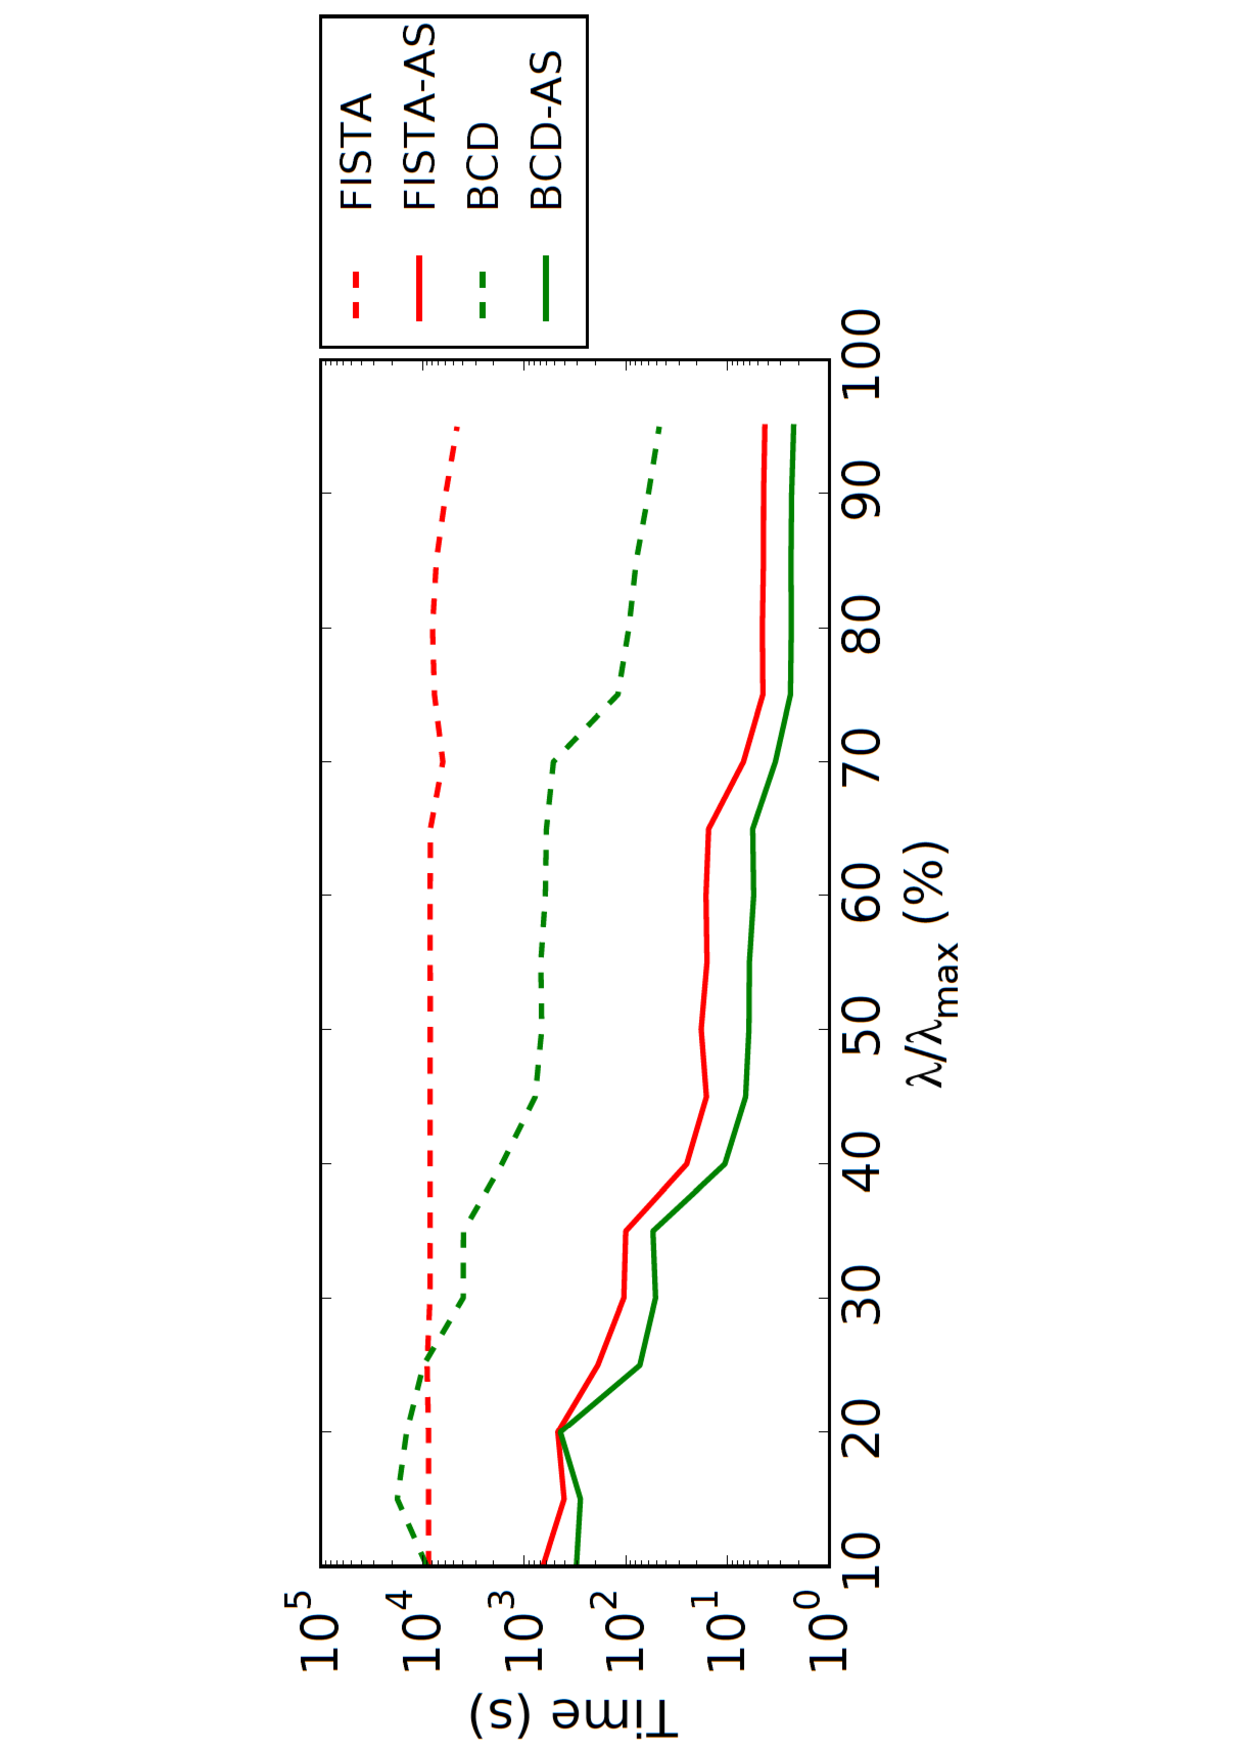
\includegraphics[trim={1cm 0.5cm 2cm 0.5cm},angle=270,width=0.95\textwidth]{background/comparison_fista_bcd}
    \caption{Computation time as a function of $\lambda$ for group LASSO on real MEG data using BCD and FISTA with (solid) and without (dashed) active set strategy.}
    \label{fig:comparison_fista_bcd}
\end{figure}

\subsection{Conclusion}
This second part demonstrated how to model the inverse problem as a regularized regression problem. It defined the multiple priors that have been used in the literature including the sparse approaches that are the main interest of this thesis. Then it introduced some of the methods for solving the different convex optimization problems. This is again not an exhaustive list and not all details have been presented here. 

So far, We have defined all the basics to understand the motivation of the sparsity priors in the M/EEG application, and also the basic tools to solve those optimization problems. Note that several points have not been introduced although very critical, which are:
\begin{itemize}
	\item The stopping criterion. The standard way is to check if the solution at iteration $k$ has not been improved more than a fixed tolerance threshold. This is an acceptable strategy, although not the best one. A more rigorous criteria would be based on the \textit{duality gap} \cite{boyd2004convex}.
    \item Screening strategies. The main challenge is not only to solve the inverse problem but also to be the least computationally demanding. Screening strategies are based on finding the most probable support of active sources in order to not do the computation for the sources that are likely to be zero (non active). This implies speeding up the convergence.
    \item Dipole orientation. As presented in Section \ref{section_dipfit}, a source is defined as a position, amplitude and orientation. Note that the orientation is not presented in the distributed section \ref{section_distributed}.
\end{itemize}
